\chapter{Amortized analysis}

\index{amortized analysis}

The time complexity of an algorithm
is often easy to analyze
just by examining the structure
of the algorithm:
what loops does the algorithm contain
and how many times the loops are performed.
However, sometimes a straightforward analysis
does not give a true picture of the efficiency of the algorithm.

\key{Amortized analysis} can be used for analyzing
algorithms that contain operations whose
time complexity varies.
The idea is to estimate the total time used for
all such operations during the
execution of the algorithm, instead of focusing
on individual operations.

\section{Two pointers method}

\index{two pointers method}

In the \key{two pointers method},
two pointers are used for
iterating through the elements in an array.
Both pointers can move during the algorithm,
but each pointer can move to one direction only.
This restriction ensures that the algorithm works efficiently.

We will next discuss two problems that can be solved
using the two pointers method.

\subsubsection{Subarray sum}

As the first example,
we consider a problem where we are
given an array of $n$ positive numbers
and a target sum $x$,
and we should find a subarray whose sum is $x$
or report that there is no such subarray.
For example, the array
\begin{center}
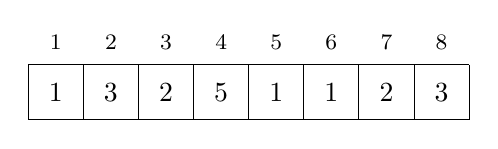
\begin{tikzpicture}[scale=0.7]
\draw (0,0) grid (8,1);

\node at (0.5,0.5) {$1$};
\node at (1.5,0.5) {$3$};
\node at (2.5,0.5) {$2$};
\node at (3.5,0.5) {$5$};
\node at (4.5,0.5) {$1$};
\node at (5.5,0.5) {$1$};
\node at (6.5,0.5) {$2$};
\node at (7.5,0.5) {$3$};

\footnotesize
\node at (0.5,1.4) {$1$};
\node at (1.5,1.4) {$2$};
\node at (2.5,1.4) {$3$};
\node at (3.5,1.4) {$4$};
\node at (4.5,1.4) {$5$};
\node at (5.5,1.4) {$6$};
\node at (6.5,1.4) {$7$};
\node at (7.5,1.4) {$8$};
\end{tikzpicture}
\end{center}
contains a subarray whose sum is 8:
\begin{center}
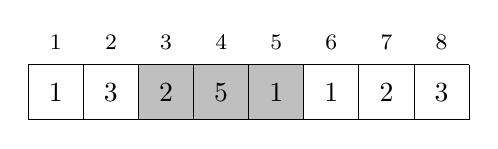
\begin{tikzpicture}[scale=0.7]
\fill[color=lightgray] (2,0) rectangle (5,1);
\draw (0,0) grid (8,1);

\node at (0.5,0.5) {$1$};
\node at (1.5,0.5) {$3$};
\node at (2.5,0.5) {$2$};
\node at (3.5,0.5) {$5$};
\node at (4.5,0.5) {$1$};
\node at (5.5,0.5) {$1$};
\node at (6.5,0.5) {$2$};
\node at (7.5,0.5) {$3$};

\footnotesize
\node at (0.5,1.4) {$1$};
\node at (1.5,1.4) {$2$};
\node at (2.5,1.4) {$3$};
\node at (3.5,1.4) {$4$};
\node at (4.5,1.4) {$5$};
\node at (5.5,1.4) {$6$};
\node at (6.5,1.4) {$7$};
\node at (7.5,1.4) {$8$};
\end{tikzpicture}
\end{center}

It turns out that the problem can be solved in
$O(n)$ time by using the two pointers method.
The idea is to use
left and right pointers that indicate the
first and last element of an subarray.
On each turn, the left pointer moves one step
forward, and the right pointer moves forward
as long as the subarray sum is at most $x$.
If the sum becomes exactly $x$,
a solution has been found.

As an example, consider the following array
with target sum $x=8$:
\begin{center}
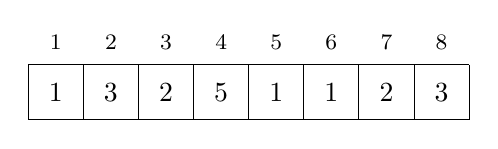
\begin{tikzpicture}[scale=0.7]
\draw (0,0) grid (8,1);

\node at (0.5,0.5) {$1$};
\node at (1.5,0.5) {$3$};
\node at (2.5,0.5) {$2$};
\node at (3.5,0.5) {$5$};
\node at (4.5,0.5) {$1$};
\node at (5.5,0.5) {$1$};
\node at (6.5,0.5) {$2$};
\node at (7.5,0.5) {$3$};

\footnotesize
\node at (0.5,1.4) {$1$};
\node at (1.5,1.4) {$2$};
\node at (2.5,1.4) {$3$};
\node at (3.5,1.4) {$4$};
\node at (4.5,1.4) {$5$};
\node at (5.5,1.4) {$6$};
\node at (6.5,1.4) {$7$};
\node at (7.5,1.4) {$8$};
\end{tikzpicture}
\end{center}

Initially, the subarray contains the elements
1, 3 and 2, and the sum of the subarray is 6.
The subarray cannot be larger, because
the next element 5 would make the sum larger than $x$.

\begin{center}
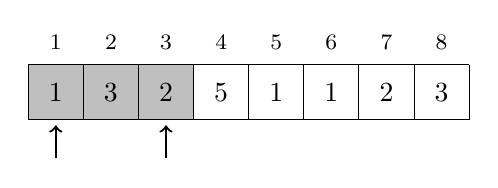
\begin{tikzpicture}[scale=0.7]
\fill[color=lightgray] (0,0) rectangle (3,1);
\draw (0,0) grid (8,1);

\node at (0.5,0.5) {$1$};
\node at (1.5,0.5) {$3$};
\node at (2.5,0.5) {$2$};
\node at (3.5,0.5) {$5$};
\node at (4.5,0.5) {$1$};
\node at (5.5,0.5) {$1$};
\node at (6.5,0.5) {$2$};
\node at (7.5,0.5) {$3$};

\draw[thick,->] (0.5,-0.7) -- (0.5,-0.1);
\draw[thick,->] (2.5,-0.7) -- (2.5,-0.1);

\footnotesize
\node at (0.5,1.4) {$1$};
\node at (1.5,1.4) {$2$};
\node at (2.5,1.4) {$3$};
\node at (3.5,1.4) {$4$};
\node at (4.5,1.4) {$5$};
\node at (5.5,1.4) {$6$};
\node at (6.5,1.4) {$7$};
\node at (7.5,1.4) {$8$};
\end{tikzpicture}
\end{center}

Then, the left pointer moves one step forward.
The right pointer does not move, because otherwise
the sum would become too large.

\begin{center}
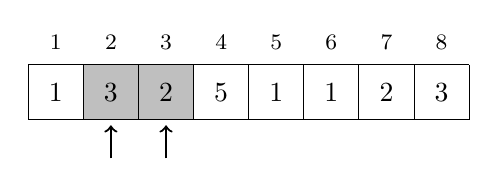
\begin{tikzpicture}[scale=0.7]
\fill[color=lightgray] (1,0) rectangle (3,1);
\draw (0,0) grid (8,1);

\node at (0.5,0.5) {$1$};
\node at (1.5,0.5) {$3$};
\node at (2.5,0.5) {$2$};
\node at (3.5,0.5) {$5$};
\node at (4.5,0.5) {$1$};
\node at (5.5,0.5) {$1$};
\node at (6.5,0.5) {$2$};
\node at (7.5,0.5) {$3$};

\draw[thick,->] (1.5,-0.7) -- (1.5,-0.1);
\draw[thick,->] (2.5,-0.7) -- (2.5,-0.1);

\footnotesize
\node at (0.5,1.4) {$1$};
\node at (1.5,1.4) {$2$};
\node at (2.5,1.4) {$3$};
\node at (3.5,1.4) {$4$};
\node at (4.5,1.4) {$5$};
\node at (5.5,1.4) {$6$};
\node at (6.5,1.4) {$7$};
\node at (7.5,1.4) {$8$};
\end{tikzpicture}
\end{center}

Again, the left pointer moves one step forward,
and this time the right pointer moves three
steps forward.
The sum is $2+5+1=8$, so we have found a subarray
where the sum of the elements is $x$.

\begin{center}
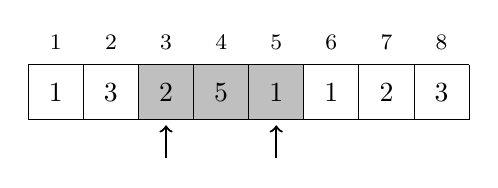
\begin{tikzpicture}[scale=0.7]
\fill[color=lightgray] (2,0) rectangle (5,1);
\draw (0,0) grid (8,1);

\node at (0.5,0.5) {$1$};
\node at (1.5,0.5) {$3$};
\node at (2.5,0.5) {$2$};
\node at (3.5,0.5) {$5$};
\node at (4.5,0.5) {$1$};
\node at (5.5,0.5) {$1$};
\node at (6.5,0.5) {$2$};
\node at (7.5,0.5) {$3$};

\draw[thick,->] (2.5,-0.7) -- (2.5,-0.1);
\draw[thick,->] (4.5,-0.7) -- (4.5,-0.1);

\footnotesize
\node at (0.5,1.4) {$1$};
\node at (1.5,1.4) {$2$};
\node at (2.5,1.4) {$3$};
\node at (3.5,1.4) {$4$};
\node at (4.5,1.4) {$5$};
\node at (5.5,1.4) {$6$};
\node at (6.5,1.4) {$7$};
\node at (7.5,1.4) {$8$};
\end{tikzpicture}
\end{center}

The time complexity of the algorithm depends on
the number of steps the right pointer moves.
There is no useful upper bound how many steps the
pointer can move on a single turn.
However, the pointer moves \emph{a total of}
$O(n)$ steps during the algorithm,
because it only moves forward.

Since both the left and right pointer
move $O(n)$ steps during the algorithm,
the time complexity is $O(n)$.

\subsubsection{2SUM problem}

\index{2SUM problem}

Another problem that can be solved using
the two pointers method is the following problem,
also known as the \key{2SUM problem}:
we are given an array of $n$ numbers and
a target sum $x$, and our task is to find two numbers
in the array such that their sum is $x$,
or report that no such numbers exist.

To solve the problem, we first
sort the numbers in the array in increasing order.
After that, we iterate through the array using
two pointers.
The left pointer starts at the first element
and moves one step forward on each turn.
The right pointer begins at the last element
and always moves backward until the sum of the
elements is at most $x$.
If the sum of the elements is exactly $x$,
a solution has been found.

For example, consider the following array
with target sum $x=12$:
\begin{center}
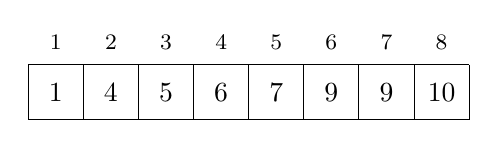
\begin{tikzpicture}[scale=0.7]
\draw (0,0) grid (8,1);

\node at (0.5,0.5) {$1$};
\node at (1.5,0.5) {$4$};
\node at (2.5,0.5) {$5$};
\node at (3.5,0.5) {$6$};
\node at (4.5,0.5) {$7$};
\node at (5.5,0.5) {$9$};
\node at (6.5,0.5) {$9$};
\node at (7.5,0.5) {$10$};

\footnotesize
\node at (0.5,1.4) {$1$};
\node at (1.5,1.4) {$2$};
\node at (2.5,1.4) {$3$};
\node at (3.5,1.4) {$4$};
\node at (4.5,1.4) {$5$};
\node at (5.5,1.4) {$6$};
\node at (6.5,1.4) {$7$};
\node at (7.5,1.4) {$8$};
\end{tikzpicture}
\end{center}

The initial positions of the pointers
are as follows.
The sum of the numbers is $1+10=11$
that is smaller than $x$.

\begin{center}
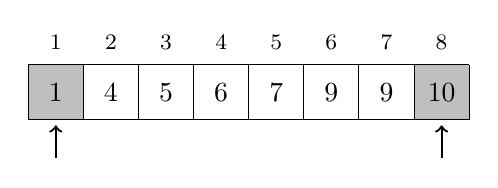
\begin{tikzpicture}[scale=0.7]
\fill[color=lightgray] (0,0) rectangle (1,1);
\fill[color=lightgray] (7,0) rectangle (8,1);
\draw (0,0) grid (8,1);

\node at (0.5,0.5) {$1$};
\node at (1.5,0.5) {$4$};
\node at (2.5,0.5) {$5$};
\node at (3.5,0.5) {$6$};
\node at (4.5,0.5) {$7$};
\node at (5.5,0.5) {$9$};
\node at (6.5,0.5) {$9$};
\node at (7.5,0.5) {$10$};

\draw[thick,->] (0.5,-0.7) -- (0.5,-0.1);
\draw[thick,->] (7.5,-0.7) -- (7.5,-0.1);

\footnotesize
\node at (0.5,1.4) {$1$};
\node at (1.5,1.4) {$2$};
\node at (2.5,1.4) {$3$};
\node at (3.5,1.4) {$4$};
\node at (4.5,1.4) {$5$};
\node at (5.5,1.4) {$6$};
\node at (6.5,1.4) {$7$};
\node at (7.5,1.4) {$8$};
\end{tikzpicture}
\end{center}

Then the left pointer moves one step forward.
The right pointer moves three steps backward,
and the sum becomes $4+7=11$.

\begin{center}
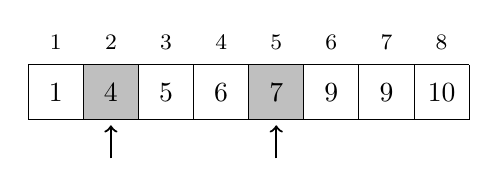
\begin{tikzpicture}[scale=0.7]
\fill[color=lightgray] (1,0) rectangle (2,1);
\fill[color=lightgray] (4,0) rectangle (5,1);
\draw (0,0) grid (8,1);

\node at (0.5,0.5) {$1$};
\node at (1.5,0.5) {$4$};
\node at (2.5,0.5) {$5$};
\node at (3.5,0.5) {$6$};
\node at (4.5,0.5) {$7$};
\node at (5.5,0.5) {$9$};
\node at (6.5,0.5) {$9$};
\node at (7.5,0.5) {$10$};

\draw[thick,->] (1.5,-0.7) -- (1.5,-0.1);
\draw[thick,->] (4.5,-0.7) -- (4.5,-0.1);

\footnotesize
\node at (0.5,1.4) {$1$};
\node at (1.5,1.4) {$2$};
\node at (2.5,1.4) {$3$};
\node at (3.5,1.4) {$4$};
\node at (4.5,1.4) {$5$};
\node at (5.5,1.4) {$6$};
\node at (6.5,1.4) {$7$};
\node at (7.5,1.4) {$8$};
\end{tikzpicture}
\end{center}

After this, the left pointer moves one step forward again.
The right pointer does not move, and a solution
$5+7=12$ has been found.

\begin{center}
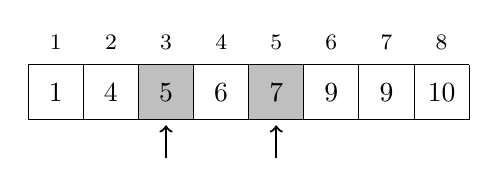
\begin{tikzpicture}[scale=0.7]
\fill[color=lightgray] (2,0) rectangle (3,1);
\fill[color=lightgray] (4,0) rectangle (5,1);
\draw (0,0) grid (8,1);

\node at (0.5,0.5) {$1$};
\node at (1.5,0.5) {$4$};
\node at (2.5,0.5) {$5$};
\node at (3.5,0.5) {$6$};
\node at (4.5,0.5) {$7$};
\node at (5.5,0.5) {$9$};
\node at (6.5,0.5) {$9$};
\node at (7.5,0.5) {$10$};

\draw[thick,->] (2.5,-0.7) -- (2.5,-0.1);
\draw[thick,->] (4.5,-0.7) -- (4.5,-0.1);

\footnotesize
\node at (0.5,1.4) {$1$};
\node at (1.5,1.4) {$2$};
\node at (2.5,1.4) {$3$};
\node at (3.5,1.4) {$4$};
\node at (4.5,1.4) {$5$};
\node at (5.5,1.4) {$6$};
\node at (6.5,1.4) {$7$};
\node at (7.5,1.4) {$8$};
\end{tikzpicture}
\end{center}

The algorithm consists of two phases:
First, sorting the array takes $O(n \log n)$ time.
After this, the left pointer moves $O(n)$ steps
forward, and the right pointer moves $O(n)$ steps
backward. Thus, the total time complexity
of the algorithm is $O(n \log n)$.

Note that it is possible to solve the problem
in another way in $O(n \log n)$ time using binary search.
In such a solution, we iterate through the array
and for each number, we try to find another
number such that the sum is $x$.
This can be done by performing $n$ binary searches,
and each search takes $O(\log n)$ time.

\index{3SUM problem}
A more difficult problem is 
the \key{3SUM problem} that asks to
find \emph{three} numbers in the array
such that their sum is $x$.
Using the idea of the above algorithm,
this problem can be solved in $O(n^2)$ time\footnote{For a long time,
it was thought that solving
the 3SUM problem more efficiently than in $O(n^2)$ time
would not be possible.
However, in 2014, it turned out \cite{gro14}
that this is not the case.}.
Can you see how?

\section{Nearest smaller elements}

\index{nearest smaller elements}

Amortized analysis is often used for
estimating the number of operations
performed on a data structure.
The operations may be distributed unevenly so
that most operations occur during a
certain phase of the algorithm, but the total
number of the operations is limited.

As an example, consider the problem
of finding for each element
of an array the
\key{nearest smaller element}, i.e.,
the first smaller element that precedes
the element in the array.
It is possible that no such element exists,
in which case the algorithm should report this.
It turns out that the problem can be solved
in $O(n)$ time using an appropriate data structure.

An efficient solution to the problem is to
iterate through the array from left to right
and maintain a chain of elements where the
first element is the current element
and each following element is the nearest smaller
element of the previous element.
If the chain only contains one element,
the current element does not have a nearest smaller element.
At each step, elements are removed from the chain
until the first element is smaller
than the current element, or the chain is empty.
After this, the current element is added to the chain.

As an example, consider the following array:
\begin{center}
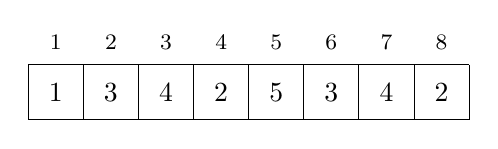
\begin{tikzpicture}[scale=0.7]
\draw (0,0) grid (8,1);

\node at (0.5,0.5) {$1$};
\node at (1.5,0.5) {$3$};
\node at (2.5,0.5) {$4$};
\node at (3.5,0.5) {$2$};
\node at (4.5,0.5) {$5$};
\node at (5.5,0.5) {$3$};
\node at (6.5,0.5) {$4$};
\node at (7.5,0.5) {$2$};

\footnotesize
\node at (0.5,1.4) {$1$};
\node at (1.5,1.4) {$2$};
\node at (2.5,1.4) {$3$};
\node at (3.5,1.4) {$4$};
\node at (4.5,1.4) {$5$};
\node at (5.5,1.4) {$6$};
\node at (6.5,1.4) {$7$};
\node at (7.5,1.4) {$8$};
\end{tikzpicture}
\end{center}

First, the numbers 1, 3 and 4 are added to the chain,
because each number is larger than the previous number.
Thus, the nearest smaller element of 4 is 3,
and the nearest smaller element of 3 is 1.
\begin{center}
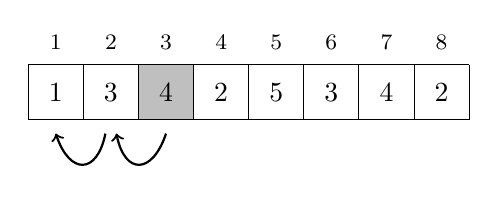
\begin{tikzpicture}[scale=0.7]
\fill[color=lightgray] (2,0) rectangle (3,1);
\draw (0,0) grid (8,1);

\node at (0.5,0.5) {$1$};
\node at (1.5,0.5) {$3$};
\node at (2.5,0.5) {$4$};
\node at (3.5,0.5) {$2$};
\node at (4.5,0.5) {$5$};
\node at (5.5,0.5) {$3$};
\node at (6.5,0.5) {$4$};
\node at (7.5,0.5) {$2$};

\draw[thick,->] (2.5,-0.25) .. controls (2.25,-1.00) and (1.75,-1.00) .. (1.6,-0.25);
\draw[thick,->] (1.4,-0.25) .. controls (1.25,-1.00) and (0.75,-1.00) .. (0.5,-0.25);

\footnotesize
\node at (0.5,1.4) {$1$};
\node at (1.5,1.4) {$2$};
\node at (2.5,1.4) {$3$};
\node at (3.5,1.4) {$4$};
\node at (4.5,1.4) {$5$};
\node at (5.5,1.4) {$6$};
\node at (6.5,1.4) {$7$};
\node at (7.5,1.4) {$8$};
\end{tikzpicture}
\end{center}

The next number 2 is smaller than the two first numbers in the chain.
Thus, the numbers 4 and 3 are removed from the chain,
and then the number 2
is added to the chain.
Its nearest smaller element is 1:
\begin{center}
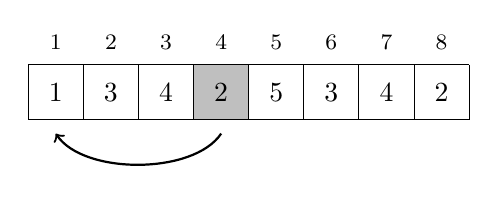
\begin{tikzpicture}[scale=0.7]
\fill[color=lightgray] (3,0) rectangle (4,1);
\draw (0,0) grid (8,1);

\node at (0.5,0.5) {$1$};
\node at (1.5,0.5) {$3$};
\node at (2.5,0.5) {$4$};
\node at (3.5,0.5) {$2$};
\node at (4.5,0.5) {$5$};
\node at (5.5,0.5) {$3$};
\node at (6.5,0.5) {$4$};
\node at (7.5,0.5) {$2$};

\draw[thick,->] (3.5,-0.25) .. controls (3.00,-1.00) and (1.00,-1.00) .. (0.5,-0.25);

\footnotesize
\node at (0.5,1.4) {$1$};
\node at (1.5,1.4) {$2$};
\node at (2.5,1.4) {$3$};
\node at (3.5,1.4) {$4$};
\node at (4.5,1.4) {$5$};
\node at (5.5,1.4) {$6$};
\node at (6.5,1.4) {$7$};
\node at (7.5,1.4) {$8$};
\end{tikzpicture}
\end{center}

After this, the number 5 is larger than the number 2,
so it will be added to the chain, and
its nearest smaller element is 2:
\begin{center}
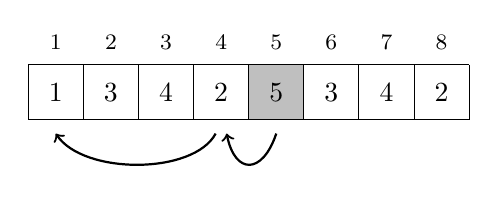
\begin{tikzpicture}[scale=0.7]
\fill[color=lightgray] (4,0) rectangle (5,1);
\draw (0,0) grid (8,1);

\node at (0.5,0.5) {$1$};
\node at (1.5,0.5) {$3$};
\node at (2.5,0.5) {$4$};
\node at (3.5,0.5) {$2$};
\node at (4.5,0.5) {$5$};
\node at (5.5,0.5) {$3$};
\node at (6.5,0.5) {$4$};
\node at (7.5,0.5) {$2$};

\draw[thick,->] (3.4,-0.25) .. controls (3.00,-1.00) and (1.00,-1.00) .. (0.5,-0.25);
\draw[thick,->] (4.5,-0.25) .. controls (4.25,-1.00) and (3.75,-1.00) .. (3.6,-0.25);

\footnotesize
\node at (0.5,1.4) {$1$};
\node at (1.5,1.4) {$2$};
\node at (2.5,1.4) {$3$};
\node at (3.5,1.4) {$4$};
\node at (4.5,1.4) {$5$};
\node at (5.5,1.4) {$6$};
\node at (6.5,1.4) {$7$};
\node at (7.5,1.4) {$8$};
\end{tikzpicture}
\end{center}

The algorithm continues in the same way
and finds the nearest smaller element
for each number in the array.
But how efficient is the algorithm?

The efficiency of the algorithm depends on
the total time used for manipulating the chain.
If an element is larger than the first
element of the chain, it is directly added
to the chain, which is efficient.
However, sometimes the chain can contain several
larger elements and it takes time to remove them.
Still, each element is added exactly once to the chain
and removed at most once from the chain.
Thus, each element causes $O(1)$ chain operations,
and the total time complexity
of the algorithm is $O(n)$.

\section{Sliding window minimum}

\index{sliding window}
\index{sliding window minimum}

A \key{sliding window} is a constant-size subarray
that moves through the array.
At each position of the window,
we want to calculate some information
about the elements inside the window.
An interesting problem is to maintain
the \key{sliding window minimum},
which means that at each position of the window,
we should report the smallest element inside the window.

The sliding window minimum can be calculated
using the same idea that we used for calculating
the nearest smaller elements.
We maintain a chain whose
first element is always the last element in the window,
and each element in the chain is smaller than the previous element.
The last element in the chain is always the
smallest element inside the window.
When the sliding window moves forward and
a new element appears, we remove from the chain
all elements that are larger than the new element.
After this, we add the new element to the chain.
Finally, if the last element in the chain
does not belong to the window anymore,
it is removed from the chain.

As an example, consider the following array:

\begin{center}
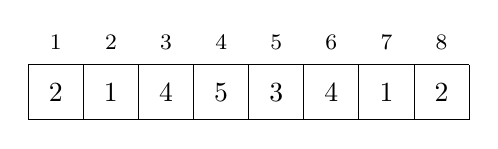
\begin{tikzpicture}[scale=0.7]
\draw (0,0) grid (8,1);

\node at (0.5,0.5) {$2$};
\node at (1.5,0.5) {$1$};
\node at (2.5,0.5) {$4$};
\node at (3.5,0.5) {$5$};
\node at (4.5,0.5) {$3$};
\node at (5.5,0.5) {$4$};
\node at (6.5,0.5) {$1$};
\node at (7.5,0.5) {$2$};

\footnotesize
\node at (0.5,1.4) {$1$};
\node at (1.5,1.4) {$2$};
\node at (2.5,1.4) {$3$};
\node at (3.5,1.4) {$4$};
\node at (4.5,1.4) {$5$};
\node at (5.5,1.4) {$6$};
\node at (6.5,1.4) {$7$};
\node at (7.5,1.4) {$8$};
\end{tikzpicture}
\end{center}

Suppose that the size of the sliding window is 4.
At the first window position, the smallest element is 1:
\begin{center}
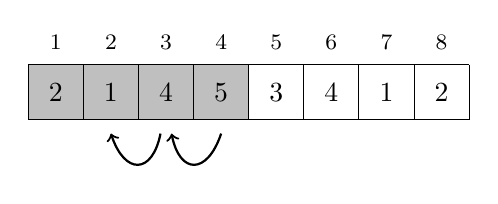
\begin{tikzpicture}[scale=0.7]
\fill[color=lightgray] (0,0) rectangle (4,1);
\draw (0,0) grid (8,1);

\node at (0.5,0.5) {$2$};
\node at (1.5,0.5) {$1$};
\node at (2.5,0.5) {$4$};
\node at (3.5,0.5) {$5$};
\node at (4.5,0.5) {$3$};
\node at (5.5,0.5) {$4$};
\node at (6.5,0.5) {$1$};
\node at (7.5,0.5) {$2$};

\footnotesize
\node at (0.5,1.4) {$1$};
\node at (1.5,1.4) {$2$};
\node at (2.5,1.4) {$3$};
\node at (3.5,1.4) {$4$};
\node at (4.5,1.4) {$5$};
\node at (5.5,1.4) {$6$};
\node at (6.5,1.4) {$7$};
\node at (7.5,1.4) {$8$};

\draw[thick,->] (3.5,-0.25) .. controls (3.25,-1.00) and (2.75,-1.00) .. (2.6,-0.25);
\draw[thick,->] (2.4,-0.25) .. controls (2.25,-1.00) and (1.75,-1.00) .. (1.5,-0.25);

\end{tikzpicture}
\end{center}

Then the window moves one step forward.
The new number 3 is smaller than the numbers
5 and 4 in the chain, so the numbers 5 and 4
are removed from the chain
and the number 3 is added to the chain.
The smallest element is still 1.
\begin{center}
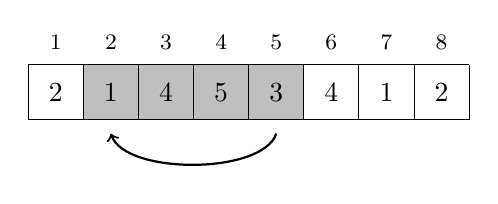
\begin{tikzpicture}[scale=0.7]
\fill[color=lightgray] (1,0) rectangle (5,1);
\draw (0,0) grid (8,1);

\node at (0.5,0.5) {$2$};
\node at (1.5,0.5) {$1$};
\node at (2.5,0.5) {$4$};
\node at (3.5,0.5) {$5$};
\node at (4.5,0.5) {$3$};
\node at (5.5,0.5) {$4$};
\node at (6.5,0.5) {$1$};
\node at (7.5,0.5) {$2$};

\footnotesize
\node at (0.5,1.4) {$1$};
\node at (1.5,1.4) {$2$};
\node at (2.5,1.4) {$3$};
\node at (3.5,1.4) {$4$};
\node at (4.5,1.4) {$5$};
\node at (5.5,1.4) {$6$};
\node at (6.5,1.4) {$7$};
\node at (7.5,1.4) {$8$};

\draw[thick,->] (4.5,-0.25) .. controls (4.25,-1.00) and (1.75,-1.00) .. (1.5,-0.25);

\end{tikzpicture}
\end{center}

After this, the window moves again,
and the smallest element 1
does not belong to the window anymore.
Thus, it is removed from the chain and the smallest
element is now 3. In addition, the new number 4
is added to the chain.
\begin{center}
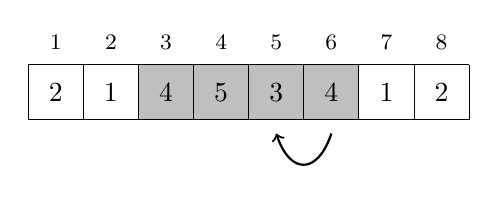
\begin{tikzpicture}[scale=0.7]
\fill[color=lightgray] (2,0) rectangle (6,1);
\draw (0,0) grid (8,1);

\node at (0.5,0.5) {$2$};
\node at (1.5,0.5) {$1$};
\node at (2.5,0.5) {$4$};
\node at (3.5,0.5) {$5$};
\node at (4.5,0.5) {$3$};
\node at (5.5,0.5) {$4$};
\node at (6.5,0.5) {$1$};
\node at (7.5,0.5) {$2$};

\footnotesize
\node at (0.5,1.4) {$1$};
\node at (1.5,1.4) {$2$};
\node at (2.5,1.4) {$3$};
\node at (3.5,1.4) {$4$};
\node at (4.5,1.4) {$5$};
\node at (5.5,1.4) {$6$};
\node at (6.5,1.4) {$7$};
\node at (7.5,1.4) {$8$};

\draw[thick,->] (5.5,-0.25) .. controls (5.25,-1.00) and (4.75,-1.00) .. (4.5,-0.25);
\end{tikzpicture}
\end{center}

The next new element 1 is smaller than all elements
in the chain.
Thus, all elements are removed from the chain
and it will only contain the element 1:
\begin{center}
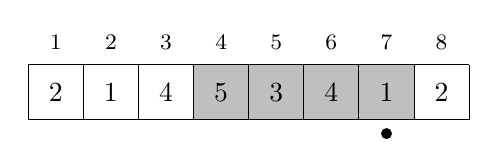
\begin{tikzpicture}[scale=0.7]
\fill[color=lightgray] (3,0) rectangle (7,1);
\draw (0,0) grid (8,1);

\node at (0.5,0.5) {$2$};
\node at (1.5,0.5) {$1$};
\node at (2.5,0.5) {$4$};
\node at (3.5,0.5) {$5$};
\node at (4.5,0.5) {$3$};
\node at (5.5,0.5) {$4$};
\node at (6.5,0.5) {$1$};
\node at (7.5,0.5) {$2$};

\footnotesize
\node at (0.5,1.4) {$1$};
\node at (1.5,1.4) {$2$};
\node at (2.5,1.4) {$3$};
\node at (3.5,1.4) {$4$};
\node at (4.5,1.4) {$5$};
\node at (5.5,1.4) {$6$};
\node at (6.5,1.4) {$7$};
\node at (7.5,1.4) {$8$};

\fill[color=black] (6.5,-0.25) circle (0.1);

%\draw[thick,->] (5.5,-0.25) .. controls (5.25,-1.00) and (4.75,-1.00) .. (4.5,-0.25);
\end{tikzpicture}
\end{center}

Finally the window reaches its last position.
The number 2 is added to the chain,
but the smallest element inside the window
is still 1.
\begin{center}
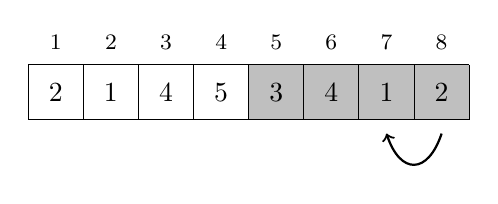
\begin{tikzpicture}[scale=0.7]
\fill[color=lightgray] (4,0) rectangle (8,1);
\draw (0,0) grid (8,1);

\node at (0.5,0.5) {$2$};
\node at (1.5,0.5) {$1$};
\node at (2.5,0.5) {$4$};
\node at (3.5,0.5) {$5$};
\node at (4.5,0.5) {$3$};
\node at (5.5,0.5) {$4$};
\node at (6.5,0.5) {$1$};
\node at (7.5,0.5) {$2$};

\footnotesize
\node at (0.5,1.4) {$1$};
\node at (1.5,1.4) {$2$};
\node at (2.5,1.4) {$3$};
\node at (3.5,1.4) {$4$};
\node at (4.5,1.4) {$5$};
\node at (5.5,1.4) {$6$};
\node at (6.5,1.4) {$7$};
\node at (7.5,1.4) {$8$};

\draw[thick,->] (7.5,-0.25) .. controls (7.25,-1.00) and (6.75,-1.00) .. (6.5,-0.25);
\end{tikzpicture}
\end{center}

Also in this algorithm, each element in the array
is added to the chain exactly once and
removed from the chain at most once.
Thus, the total time complexity of the algorithm is $O(n)$.



